% Options for packages loaded elsewhere
\PassOptionsToPackage{unicode}{hyperref}
\PassOptionsToPackage{hyphens}{url}
\PassOptionsToPackage{dvipsnames,svgnames,x11names}{xcolor}
%
\documentclass[
]{book}
\usepackage{amsmath,amssymb}
\usepackage{iftex}
\ifPDFTeX
  \usepackage[T1]{fontenc}
  \usepackage[utf8]{inputenc}
  \usepackage{textcomp} % provide euro and other symbols
\else % if luatex or xetex
  \usepackage{unicode-math} % this also loads fontspec
  \defaultfontfeatures{Scale=MatchLowercase}
  \defaultfontfeatures[\rmfamily]{Ligatures=TeX,Scale=1}
\fi
\usepackage{lmodern}
\ifPDFTeX\else
  % xetex/luatex font selection
\fi
% Use upquote if available, for straight quotes in verbatim environments
\IfFileExists{upquote.sty}{\usepackage{upquote}}{}
\IfFileExists{microtype.sty}{% use microtype if available
  \usepackage[]{microtype}
  \UseMicrotypeSet[protrusion]{basicmath} % disable protrusion for tt fonts
}{}
\makeatletter
\@ifundefined{KOMAClassName}{% if non-KOMA class
  \IfFileExists{parskip.sty}{%
    \usepackage{parskip}
  }{% else
    \setlength{\parindent}{0pt}
    \setlength{\parskip}{6pt plus 2pt minus 1pt}}
}{% if KOMA class
  \KOMAoptions{parskip=half}}
\makeatother
\usepackage{xcolor}
\usepackage{color}
\usepackage{fancyvrb}
\newcommand{\VerbBar}{|}
\newcommand{\VERB}{\Verb[commandchars=\\\{\}]}
\DefineVerbatimEnvironment{Highlighting}{Verbatim}{commandchars=\\\{\}}
% Add ',fontsize=\small' for more characters per line
\usepackage{framed}
\definecolor{shadecolor}{RGB}{248,248,248}
\newenvironment{Shaded}{\begin{snugshade}}{\end{snugshade}}
\newcommand{\AlertTok}[1]{\textcolor[rgb]{0.94,0.16,0.16}{#1}}
\newcommand{\AnnotationTok}[1]{\textcolor[rgb]{0.56,0.35,0.01}{\textbf{\textit{#1}}}}
\newcommand{\AttributeTok}[1]{\textcolor[rgb]{0.13,0.29,0.53}{#1}}
\newcommand{\BaseNTok}[1]{\textcolor[rgb]{0.00,0.00,0.81}{#1}}
\newcommand{\BuiltInTok}[1]{#1}
\newcommand{\CharTok}[1]{\textcolor[rgb]{0.31,0.60,0.02}{#1}}
\newcommand{\CommentTok}[1]{\textcolor[rgb]{0.56,0.35,0.01}{\textit{#1}}}
\newcommand{\CommentVarTok}[1]{\textcolor[rgb]{0.56,0.35,0.01}{\textbf{\textit{#1}}}}
\newcommand{\ConstantTok}[1]{\textcolor[rgb]{0.56,0.35,0.01}{#1}}
\newcommand{\ControlFlowTok}[1]{\textcolor[rgb]{0.13,0.29,0.53}{\textbf{#1}}}
\newcommand{\DataTypeTok}[1]{\textcolor[rgb]{0.13,0.29,0.53}{#1}}
\newcommand{\DecValTok}[1]{\textcolor[rgb]{0.00,0.00,0.81}{#1}}
\newcommand{\DocumentationTok}[1]{\textcolor[rgb]{0.56,0.35,0.01}{\textbf{\textit{#1}}}}
\newcommand{\ErrorTok}[1]{\textcolor[rgb]{0.64,0.00,0.00}{\textbf{#1}}}
\newcommand{\ExtensionTok}[1]{#1}
\newcommand{\FloatTok}[1]{\textcolor[rgb]{0.00,0.00,0.81}{#1}}
\newcommand{\FunctionTok}[1]{\textcolor[rgb]{0.13,0.29,0.53}{\textbf{#1}}}
\newcommand{\ImportTok}[1]{#1}
\newcommand{\InformationTok}[1]{\textcolor[rgb]{0.56,0.35,0.01}{\textbf{\textit{#1}}}}
\newcommand{\KeywordTok}[1]{\textcolor[rgb]{0.13,0.29,0.53}{\textbf{#1}}}
\newcommand{\NormalTok}[1]{#1}
\newcommand{\OperatorTok}[1]{\textcolor[rgb]{0.81,0.36,0.00}{\textbf{#1}}}
\newcommand{\OtherTok}[1]{\textcolor[rgb]{0.56,0.35,0.01}{#1}}
\newcommand{\PreprocessorTok}[1]{\textcolor[rgb]{0.56,0.35,0.01}{\textit{#1}}}
\newcommand{\RegionMarkerTok}[1]{#1}
\newcommand{\SpecialCharTok}[1]{\textcolor[rgb]{0.81,0.36,0.00}{\textbf{#1}}}
\newcommand{\SpecialStringTok}[1]{\textcolor[rgb]{0.31,0.60,0.02}{#1}}
\newcommand{\StringTok}[1]{\textcolor[rgb]{0.31,0.60,0.02}{#1}}
\newcommand{\VariableTok}[1]{\textcolor[rgb]{0.00,0.00,0.00}{#1}}
\newcommand{\VerbatimStringTok}[1]{\textcolor[rgb]{0.31,0.60,0.02}{#1}}
\newcommand{\WarningTok}[1]{\textcolor[rgb]{0.56,0.35,0.01}{\textbf{\textit{#1}}}}
\usepackage{longtable,booktabs,array}
\usepackage{calc} % for calculating minipage widths
% Correct order of tables after \paragraph or \subparagraph
\usepackage{etoolbox}
\makeatletter
\patchcmd\longtable{\par}{\if@noskipsec\mbox{}\fi\par}{}{}
\makeatother
% Allow footnotes in longtable head/foot
\IfFileExists{footnotehyper.sty}{\usepackage{footnotehyper}}{\usepackage{footnote}}
\makesavenoteenv{longtable}
\usepackage{graphicx}
\makeatletter
\def\maxwidth{\ifdim\Gin@nat@width>\linewidth\linewidth\else\Gin@nat@width\fi}
\def\maxheight{\ifdim\Gin@nat@height>\textheight\textheight\else\Gin@nat@height\fi}
\makeatother
% Scale images if necessary, so that they will not overflow the page
% margins by default, and it is still possible to overwrite the defaults
% using explicit options in \includegraphics[width, height, ...]{}
\setkeys{Gin}{width=\maxwidth,height=\maxheight,keepaspectratio}
% Set default figure placement to htbp
\makeatletter
\def\fps@figure{htbp}
\makeatother
\setlength{\emergencystretch}{3em} % prevent overfull lines
\providecommand{\tightlist}{%
  \setlength{\itemsep}{0pt}\setlength{\parskip}{0pt}}
\setcounter{secnumdepth}{5}
\usepackage{booktabs}

\newenvironment{rmdblock}[1]
  {\begin{shaded*}
  \begin{itemize}
  \renewcommand{\labelitemi}{
    \raisebox{-.7\height}[0pt][0pt]{
      {\setkeys{Gin}{width=3em,keepaspectratio}\includegraphics{images/#1}}
    }
  }
  \item
  }
  {
  \end{itemize}
  \end{shaded*}
  }
\newenvironment{rmdnote}
  {\begin{rmdblock}{note}}
  {\end{rmdblock}}
\newenvironment{rmdtip}
  {\begin{rmdblock}{tip}}
  {\end{rmdblock}}
\newenvironment{rmdwarning}
  {\begin{rmdblock}{warning}}
  {\end{rmdblock}}
\ifLuaTeX
  \usepackage{selnolig}  % disable illegal ligatures
\fi
\usepackage[]{natbib}
\bibliographystyle{apalike}
\usepackage{bookmark}
\IfFileExists{xurl.sty}{\usepackage{xurl}}{} % add URL line breaks if available
\urlstyle{same}
% Make links footnotes instead of hotlinks:
\DeclareRobustCommand{\href}[2]{#2\footnote{\url{#1}}}
\hypersetup{
  pdftitle={GWAS Tutorial},
  pdfauthor={Yen-Hsiang (Teddy) Huang},
  colorlinks=true,
  linkcolor={Maroon},
  filecolor={Maroon},
  citecolor={Blue},
  urlcolor={Blue},
  pdfcreator={LaTeX via pandoc}}

\title{GWAS Tutorial}
\usepackage{etoolbox}
\makeatletter
\providecommand{\subtitle}[1]{% add subtitle to \maketitle
  \apptocmd{\@title}{\par {\large #1 \par}}{}{}
}
\makeatother
\subtitle{For Anaerobic Germination in Rice}
\author{Yen-Hsiang (Teddy) Huang}
\date{2024-12-16}

\begin{document}
\maketitle

{
\hypersetup{linkcolor=}
\setcounter{tocdepth}{1}
\tableofcontents
}
\chapter*{Welcome to GWAS Tutorial}\label{welcome-to-gwas-tutorial}
\addcontentsline{toc}{chapter}{Welcome to GWAS Tutorial}

This is the \href{http://tidytextmining.com/}{website} for \textbf{\emph{GWAS analysis with R and PLINK programs}}.

This work by \textbf{Yen-Hsiang (Teddy) Huang} is licensed under a GNU General Public License.


\includegraphics{images/clipboard-3960043298.png}

\chapter*{Preface}\label{preface}
\addcontentsline{toc}{chapter}{Preface}

If you work in analytics or data science, like we do, you are familiar with the fact that data is being generated all the time at ever faster rates. (You may even be a little weary of people pontificating about this fact.) Analysts are often trained to handle tabular or rectangular data that is mostly numeric, but much of the data proliferating today is unstructured and text-heavy. Many of us who work in analytical fields are not trained in even simple interpretation of natural language.

We developed the \href{https://github.com/juliasilge/tidytext}{tidytext} \citep{R-tidytext} R package because we were familiar with many methods for data wrangling and visualization, but couldn't easily apply these same methods to text. We found that using tidy data principles can make many text mining tasks easier, more effective, and consistent with tools already in wide use. Treating text as data frames of individual words allows us to manipulate, summarize, and visualize the characteristics of text easily and integrate natural language processing into effective workflows we were already using.

This book serves as an introduction of text mining using the tidytext package and other tidy tools in R. The functions provided by the tidytext package are relatively simple; what is important are the possible applications. Thus, this book provides compelling examples of real text mining problems.

\section*{Outline}\label{outline}
\addcontentsline{toc}{section}{Outline}

We start by introducing the tidy text format, and some of the ways dplyr, tidyr, and tidytext allow informative analyses of this structure.

\begin{itemize}
\tightlist
\item
  \textbf{Chapter} \ref{tidytext} outlines the tidy text format and the \texttt{unnest\_tokens()} function. It also introduces the gutenbergr and janeaustenr packages, which provide useful literary text datasets that we'll use throughout this book.
\item
  \textbf{Chapter} \ref{sentiment} shows how to perform sentiment analysis on a tidy text dataset, using the \texttt{sentiments} dataset from tidytext and \texttt{inner\_join()} from dplyr.
\item
  \textbf{Chapter} \ref{tfidf} describes the tf-idf statistic (term frequency times inverse document frequency), a quantity used for identifying terms that are especially important to a particular document.
\item
  \textbf{Chapter} \ref{ngrams} introduces n-grams and how to analyze word networks in text using the widyr and ggraph packages.
\end{itemize}

Text won't be tidy at all stages of an analysis, and it is important to be able to convert back and forth between tidy and non-tidy formats.

\begin{itemize}
\tightlist
\item
  \textbf{Chapter} \ref{dtm} introduces methods for tidying document-term matrices and corpus objects from the tm and quanteda packages, as well as for casting tidy text datasets into those formats.
\item
  \textbf{Chapter} \ref{topicmodeling} explores the concept of topic modeling, and uses the \texttt{tidy()} method to interpret and visualize the output of the topicmodels package.
\end{itemize}

We conclude with several case studies that bring together multiple tidy text mining approaches we've learned.

\begin{itemize}
\tightlist
\item
  \textbf{Chapter} \ref{twitter} demonstrates an application of a tidy text analysis by analyzing the authors' own Twitter archives. How do Dave's and Julia's tweeting habits compare?
\item
  \textbf{Chapter} \ref{nasa} explores metadata from over 32,000 NASA datasets (available in JSON) by looking at how keywords from the datasets are connected to title and description fields.
\item
  \textbf{Chapter} \ref{usenet} analyzes a dataset of Usenet messages from a diverse set of newsgroups (focused on topics like politics, hockey, technology, atheism, and more) to understand patterns across the groups.
\end{itemize}

\section*{About this book}\label{about-this-book}
\addcontentsline{toc}{section}{About this book}

This book is focused on practical software examples and data explorations. There are few equations, but a great deal of code. We especially focus on generating real insights from the literature, news, and social media that we analyze.

We don't assume any previous knowledge of text mining. Professional linguists and text analysts will likely find our examples elementary, though we are confident they can build on the framework for their own analyses.

We do assume that the reader is at least slightly familiar with dplyr, ggplot2, and the \texttt{\%\textgreater{}\%} ``pipe'' operator in R, and is interested in applying these tools to text data. For users who don't have this background, we recommend books such as \href{http://r4ds.had.co.nz/}{R for Data Science}. We believe that with a basic background and interest in tidy data, even a user early in their R career can understand and apply our examples.

\section*{Using code examples}\label{using-code-examples}
\addcontentsline{toc}{section}{Using code examples}

This book was written in \href{http://www.rstudio.com/ide/}{RStudio} using \href{http://bookdown.org/}{bookdown}. The \href{https://www.tidytextmining.com/}{website} is hosted via \href{http://netlify.com/}{Netlify}, and automatically built after every push by \href{https://help.github.com/actions}{GitHub Actions}. While we show the code behind the vast majority of the analyses, in the interest of space we sometimes choose not to show the code generating a particular visualization if we've already provided the code for several similar graphs. We trust the reader can learn from and build on our examples, and the code used to generate the book can be found in our \href{https://github.com/dgrtwo/tidy-text-mining}{public GitHub repository}. We generated all plots in this book using \href{https://ggplot2.tidyverse.org/}{ggplot2} and its light theme (\texttt{theme\_light()}).

This version of the book was built with R version 4.4.1 (2024-06-14 ucrt) and the following packages:

\begin{longtable}[]{@{}lll@{}}
\toprule\noalign{}
package & version & source \\
\midrule\noalign{}
\endhead
\bottomrule\noalign{}
\endlastfoot
bookdown & 0.40 & CRAN (R 4.4.1) \\
dplyr & 1.1.4 & CRAN (R 4.4.1) \\
forcats & 1.0.0 & CRAN (R 4.4.1) \\
ggforce & 0.4.2 & CRAN (R 4.4.1) \\
ggplot2 & 3.5.1 & CRAN (R 4.4.1) \\
ggraph & 2.2.1 & CRAN (R 4.4.1) \\
gutenbergr & NA & NA \\
igraph & 2.1.1 & CRAN (R 4.4.1) \\
janeaustenr & 1.0.0 & CRAN (R 4.4.1) \\
jsonlite & 1.8.9 & CRAN (R 4.4.2) \\
lubridate & 1.9.3 & CRAN (R 4.4.1) \\
mallet & NA & NA \\
Matrix & 1.7-0 & CRAN (R 4.4.0) \\
quanteda & NA & NA \\
readr & 2.1.5 & CRAN (R 4.4.1) \\
reshape2 & 1.4.4 & CRAN (R 4.4.1) \\
sessioninfo & 1.2.2 & CRAN (R 4.4.1) \\
stringr & 1.5.1 & CRAN (R 4.4.1) \\
styler & 1.10.3 & CRAN (R 4.4.1) \\
textdata & NA & NA \\
tidyr & 1.3.1 & CRAN (R 4.4.1) \\
tidytext & 0.4.2 & CRAN (R 4.4.1) \\
tidyverse & 2.0.0 & CRAN (R 4.4.1) \\
tm & NA & NA \\
topicmodels & NA & NA \\
widyr & NA & NA \\
wordcloud & 2.6 & CRAN (R 4.4.2) \\
XML & 3.99-0.17 & CRAN (R 4.4.1) \\
\end{longtable}

\section*{Acknowledgements}\label{acknowledgements}
\addcontentsline{toc}{section}{Acknowledgements}

We are so thankful for the contributions, help, and perspectives of people who have moved us forward in this project. There are several people and organizations we would like to thank in particular.

We would like to thank Os Keyes and Gabriela de Queiroz for their contributions to the tidytext package, Lincoln Mullen for his work on the \href{https://github.com/ropensci/tokenizers}{tokenizers} package, Kenneth Benoit for his work on the \href{https://github.com/kbenoit/quanteda}{quanteda} package, Thomas Pedersen for his work on the \href{https://github.com/thomasp85/ggraph}{ggraph} package, and Hadley Wickham for his work in framing tidy data principles and building tidy tools. We would also like to thank \href{https://ropensci.org/}{rOpenSci}, which hosted us at the unconference where we began work, and the \href{https://open.nasa.gov/explore/datanauts/}{NASA Datanauts} program, for the opportunities and support they have provided Julia during her time with them.

We received thoughtful, thorough technical reviews that improved the quality of this book significantly. We would like to thank Mara Averick, Carolyn Clayton, Simon Jackson, Sean Kross, and Lincoln Mullen for their investment of time and energy in these technical reviews.

Finally, we want to dedicate this book to our spouses, Robert and Dana. We both could produce a great deal of sentimental text on this subject but will restrict ourselves to heartfelt thanks.

\chapter{Genotype Data}\label{tidytext}

\begin{enumerate}
\def\labelenumi{\arabic{enumi}.}
\item
  \textbf{Download Rice SNP data from SNP-Seek (3K RG):} We utilized the 3K RG 18 million Base SNP Dataset and the 3K RG 404k Core SNP Dataset.
\item
  \textbf{Align Accession IDs:} Match the accession IDs between the phenotypic and SNP datasets.
\item
  \textbf{SNP Data Processing and Quality Control:} Perform data generation and quality control on the SNP data for the subset of 311 samples.
\item
  \textbf{Generate Final Genotypic Dataset:} Prepare the final genotypic dataset for GWAS analysis.
\end{enumerate}

\section{\texorpdfstring{\textbf{Download Rice SNP data from SNP-Seek (3K RG)}}{Download Rice SNP data from SNP-Seek (3K RG)}}\label{download-rice-snp-data-from-snp-seek-3k-rg}

As we stated above, we define the tidy text format as being a table with \textbf{one-token-per-row.} Structuring text data in this way means that it conforms to tidy data principles and can be manipulated with a set of consistent tools. This is worth contrasting with the ways text is often stored in text mining approaches.

\begin{itemize}
\tightlist
\item
  \textbf{String}: Text can, of course, be stored as strings, i.e., character vectors, within R, and often text data is first read into memory in this form.
\item
  \textbf{Corpus}: These types of objects typically contain raw strings annotated with additional metadata and details.
\item
  \textbf{Document-term matrix}: This is a sparse matrix describing a collection (i.e., a corpus) of documents with one row for each document and one column for each term. The value in the matrix is typically word count or tf-idf (see Chapter \ref{tfidf}).
\end{itemize}

Let's hold off on exploring corpus and document-term matrix objects until Chapter \ref{dtm}, and get down to the basics of converting text to a tidy format.

\section{\texorpdfstring{\textbf{Align Accession IDs}}{Align Accession IDs}}\label{align-accession-ids}

Emily Dickinson wrote some lovely text in her time.

\begin{Shaded}
\begin{Highlighting}[]
\NormalTok{text }\OtherTok{\textless{}{-}} \FunctionTok{c}\NormalTok{(}\StringTok{"Because I could not stop for Death {-}"}\NormalTok{,}
          \StringTok{"He kindly stopped for me {-}"}\NormalTok{,}
          \StringTok{"The Carriage held but just Ourselves {-}"}\NormalTok{,}
          \StringTok{"and Immortality"}\NormalTok{)}

\NormalTok{text}
\CommentTok{\#\textgreater{} [1] "Because I could not stop for Death {-}"  }
\CommentTok{\#\textgreater{} [2] "He kindly stopped for me {-}"            }
\CommentTok{\#\textgreater{} [3] "The Carriage held but just Ourselves {-}"}
\CommentTok{\#\textgreater{} [4] "and Immortality"}
\end{Highlighting}
\end{Shaded}

This is a typical character vector that we might want to analyze. In order to turn it into a tidy text dataset, we first need to put it into a data frame.

\begin{Shaded}
\begin{Highlighting}[]
\FunctionTok{library}\NormalTok{(dplyr)}
\NormalTok{text\_df }\OtherTok{\textless{}{-}} \FunctionTok{tibble}\NormalTok{(}\AttributeTok{line =} \DecValTok{1}\SpecialCharTok{:}\DecValTok{4}\NormalTok{, }\AttributeTok{text =}\NormalTok{ text)}

\NormalTok{text\_df}
\CommentTok{\#\textgreater{} \# A tibble: 4 x 2}
\CommentTok{\#\textgreater{}    line text                                  }
\CommentTok{\#\textgreater{}   \textless{}int\textgreater{} \textless{}chr\textgreater{}                                 }
\CommentTok{\#\textgreater{} 1     1 Because I could not stop for Death {-}  }
\CommentTok{\#\textgreater{} 2     2 He kindly stopped for me {-}            }
\CommentTok{\#\textgreater{} 3     3 The Carriage held but just Ourselves {-}}
\CommentTok{\#\textgreater{} 4     4 and Immortality}
\end{Highlighting}
\end{Shaded}

What does it mean that this data frame has printed out as a ``tibble''? A tibble is a modern class of data frame within R, available in the dplyr and tibble packages, that has a convenient print method, will not convert strings to factors, and does not use row names. Tibbles are great for use with tidy tools.

Notice that this data frame containing text isn't yet compatible with tidy text analysis, though. We can't filter out words or count which occur most frequently, since each row is made up of multiple combined words. We need to convert this so that it has \textbf{one-token-per-document-per-row}.

\begin{rmdnote}
A token is a meaningful unit of text, most often a word, that we are
interested in using for further analysis, and tokenization is the
process of splitting text into tokens.
\end{rmdnote}

In this first example, we only have one document (the poem), but we will explore examples with multiple documents soon.

Within our tidy text framework, we need to both break the text into individual tokens (a process called \emph{tokenization}) \emph{and} transform it to a tidy data structure. To do this, we use tidytext's \texttt{unnest\_tokens()} function.

\begin{Shaded}
\begin{Highlighting}[]
\FunctionTok{library}\NormalTok{(tidytext)}

\NormalTok{text\_df }\SpecialCharTok{\%\textgreater{}\%}
  \FunctionTok{unnest\_tokens}\NormalTok{(word, text)}
\CommentTok{\#\textgreater{} \# A tibble: 20 x 2}
\CommentTok{\#\textgreater{}     line word   }
\CommentTok{\#\textgreater{}    \textless{}int\textgreater{} \textless{}chr\textgreater{}  }
\CommentTok{\#\textgreater{}  1     1 because}
\CommentTok{\#\textgreater{}  2     1 i      }
\CommentTok{\#\textgreater{}  3     1 could  }
\CommentTok{\#\textgreater{}  4     1 not    }
\CommentTok{\#\textgreater{}  5     1 stop   }
\CommentTok{\#\textgreater{}  6     1 for    }
\CommentTok{\#\textgreater{}  7     1 death  }
\CommentTok{\#\textgreater{}  8     2 he     }
\CommentTok{\#\textgreater{}  9     2 kindly }
\CommentTok{\#\textgreater{} 10     2 stopped}
\CommentTok{\#\textgreater{} \# i 10 more rows}
\end{Highlighting}
\end{Shaded}

dard set of tidy tools, namely dplyr, tidyr, and ggplot2, as shown in Figure \ref{fig:tidyflow-ch1}.

\begin{figure}

{\centering 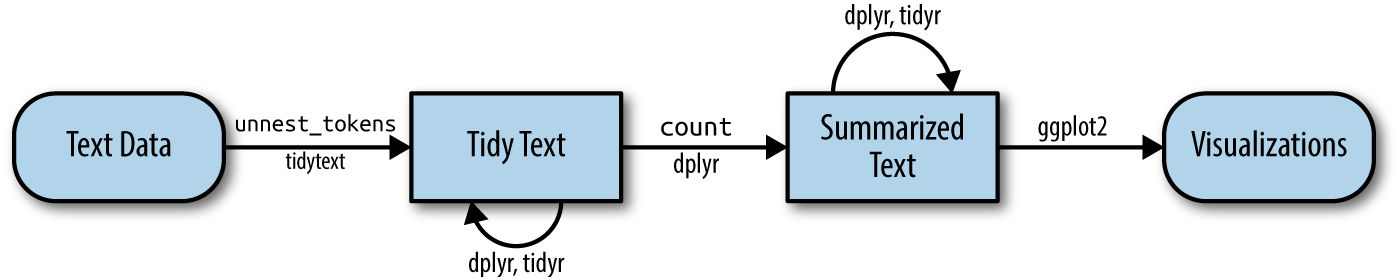
\includegraphics[width=1\linewidth]{images/tmwr_0101} 

}

\caption{A flowchart of a typical text analysis using tidy data principles. This chapter shows how to summarize and visualize text using these tools.}\label{fig:tidyflow-ch1}
\end{figure}

\section{\texorpdfstring{\textbf{SNP Data Processing and Quality Control}}{SNP Data Processing and Quality Control}}\label{tidyausten}

Let's use the text of Jane Austen's 6 completed, published novels from the \href{https://cran.r-project.org/package=janeaustenr}{janeaustenr} package \citep{R-janeaustenr}, and transform them into a tidy format. The janeaustenr package provides these texts in a one-row-per-line format, where a line in this context is analogous to a literal printed line in a physical book. Let's start with that, and also use \texttt{mutate()} to annotate a \texttt{linenumber} quantity to keep track of lines in the original format and a \texttt{chapter} (using a regex) to find where all the chapters are.

\begin{Shaded}
\begin{Highlighting}[]
\FunctionTok{library}\NormalTok{(janeaustenr)}
\FunctionTok{library}\NormalTok{(dplyr)}
\FunctionTok{library}\NormalTok{(stringr)}

\NormalTok{original\_books }\OtherTok{\textless{}{-}} \FunctionTok{austen\_books}\NormalTok{() }\SpecialCharTok{\%\textgreater{}\%}
  \FunctionTok{group\_by}\NormalTok{(book) }\SpecialCharTok{\%\textgreater{}\%}
  \FunctionTok{mutate}\NormalTok{(}\AttributeTok{linenumber =} \FunctionTok{row\_number}\NormalTok{(),}
         \AttributeTok{chapter =} \FunctionTok{cumsum}\NormalTok{(}\FunctionTok{str\_detect}\NormalTok{(text, }
                                     \FunctionTok{regex}\NormalTok{(}\StringTok{"\^{}chapter [}\SpecialCharTok{\textbackslash{}\textbackslash{}}\StringTok{divxlc]"}\NormalTok{,}
                                           \AttributeTok{ignore\_case =} \ConstantTok{TRUE}\NormalTok{)))) }\SpecialCharTok{\%\textgreater{}\%}
  \FunctionTok{ungroup}\NormalTok{()}

\NormalTok{original\_books}
\CommentTok{\#\textgreater{} \# A tibble: 73,422 x 4}
\CommentTok{\#\textgreater{}    text                    book                linenumber chapter}
\CommentTok{\#\textgreater{}    \textless{}chr\textgreater{}                   \textless{}fct\textgreater{}                    \textless{}int\textgreater{}   \textless{}int\textgreater{}}
\CommentTok{\#\textgreater{}  1 "SENSE AND SENSIBILITY" Sense \& Sensibility          1       0}
\CommentTok{\#\textgreater{}  2 ""                      Sense \& Sensibility          2       0}
\CommentTok{\#\textgreater{}  3 "by Jane Austen"        Sense \& Sensibility          3       0}
\CommentTok{\#\textgreater{}  4 ""                      Sense \& Sensibility          4       0}
\CommentTok{\#\textgreater{}  5 "(1811)"                Sense \& Sensibility          5       0}
\CommentTok{\#\textgreater{}  6 ""                      Sense \& Sensibility          6       0}
\CommentTok{\#\textgreater{}  7 ""                      Sense \& Sensibility          7       0}
\CommentTok{\#\textgreater{}  8 ""                      Sense \& Sensibility          8       0}
\CommentTok{\#\textgreater{}  9 ""                      Sense \& Sensibility          9       0}
\CommentTok{\#\textgreater{} 10 "CHAPTER 1"             Sense \& Sensibility         10       1}
\CommentTok{\#\textgreater{} \# i 73,412 more rows}
\end{Highlighting}
\end{Shaded}

To work with this as a tidy dataset, we need to restructure it in the \textbf{one-token-per-row} format, which as we saw earlier is done with the \texttt{unnest\_tokens()} function.

\begin{Shaded}
\begin{Highlighting}[]
\FunctionTok{library}\NormalTok{(tidytext)}
\NormalTok{tidy\_books }\OtherTok{\textless{}{-}}\NormalTok{ original\_books }\SpecialCharTok{\%\textgreater{}\%}
  \FunctionTok{unnest\_tokens}\NormalTok{(word, text)}

\NormalTok{tidy\_books}
\CommentTok{\#\textgreater{} \# A tibble: 725,055 x 4}
\CommentTok{\#\textgreater{}    book                linenumber chapter word       }
\CommentTok{\#\textgreater{}    \textless{}fct\textgreater{}                    \textless{}int\textgreater{}   \textless{}int\textgreater{} \textless{}chr\textgreater{}      }
\CommentTok{\#\textgreater{}  1 Sense \& Sensibility          1       0 sense      }
\CommentTok{\#\textgreater{}  2 Sense \& Sensibility          1       0 and        }
\CommentTok{\#\textgreater{}  3 Sense \& Sensibility          1       0 sensibility}
\CommentTok{\#\textgreater{}  4 Sense \& Sensibility          3       0 by         }
\CommentTok{\#\textgreater{}  5 Sense \& Sensibility          3       0 jane       }
\CommentTok{\#\textgreater{}  6 Sense \& Sensibility          3       0 austen     }
\CommentTok{\#\textgreater{}  7 Sense \& Sensibility          5       0 1811       }
\CommentTok{\#\textgreater{}  8 Sense \& Sensibility         10       1 chapter    }
\CommentTok{\#\textgreater{}  9 Sense \& Sensibility         10       1 1          }
\CommentTok{\#\textgreater{} 10 Sense \& Sensibility         13       1 the        }
\CommentTok{\#\textgreater{} \# i 725,045 more rows}
\end{Highlighting}
\end{Shaded}

This function uses the \href{https://github.com/ropensci/tokenizers}{tokenizers} package to separate each line of text in the original data frame into tokens. The default tokenizing is for words, but other options include characters, n-grams, sentences, lines, paragraphs, or separation around a regex pattern.

Now that the data is in one-word-per-row format, we can manipulate it with tidy tools like dplyr. Often in text analysis, we will want to remove stop words; stop words are words that are not useful for an analysis, typically extremely common words such as ``the'', ``of'', ``to'', and so forth in English. We can remove stop words (kept in the tidytext dataset \texttt{stop\_words}) with an \texttt{anti\_join()}.

\begin{Shaded}
\begin{Highlighting}[]
\FunctionTok{data}\NormalTok{(stop\_words)}

\NormalTok{tidy\_books }\OtherTok{\textless{}{-}}\NormalTok{ tidy\_books }\SpecialCharTok{\%\textgreater{}\%}
  \FunctionTok{anti\_join}\NormalTok{(stop\_words)}
\end{Highlighting}
\end{Shaded}

The \texttt{stop\_words} dataset in the tidytext package contains stop words from three lexicons. We can use them all together, as we have here, or \texttt{filter()} to only use one set of stop words if that is more appropriate for a certain analysis.

We can also use dplyr's \texttt{count()} to find the most common words in all the books as a whole.

\begin{Shaded}
\begin{Highlighting}[]
\NormalTok{tidy\_books }\SpecialCharTok{\%\textgreater{}\%}
  \FunctionTok{count}\NormalTok{(word, }\AttributeTok{sort =} \ConstantTok{TRUE}\NormalTok{) }
\CommentTok{\#\textgreater{} \# A tibble: 13,914 x 2}
\CommentTok{\#\textgreater{}    word       n}
\CommentTok{\#\textgreater{}    \textless{}chr\textgreater{}  \textless{}int\textgreater{}}
\CommentTok{\#\textgreater{}  1 miss    1855}
\CommentTok{\#\textgreater{}  2 time    1337}
\CommentTok{\#\textgreater{}  3 fanny    862}
\CommentTok{\#\textgreater{}  4 dear     822}
\CommentTok{\#\textgreater{}  5 lady     817}
\CommentTok{\#\textgreater{}  6 sir      806}
\CommentTok{\#\textgreater{}  7 day      797}
\CommentTok{\#\textgreater{}  8 emma     787}
\CommentTok{\#\textgreater{}  9 sister   727}
\CommentTok{\#\textgreater{} 10 house    699}
\CommentTok{\#\textgreater{} \# i 13,904 more rows}
\end{Highlighting}
\end{Shaded}

Because we've been using tidy tools, our word counts are stored in a tidy data frame. This allows us to pipe this directly to the ggplot2 package, for example to create a visualization of the most common words (Figure \ref{fig:plotcount}).

\begin{Shaded}
\begin{Highlighting}[]
\FunctionTok{library}\NormalTok{(ggplot2)}

\NormalTok{tidy\_books }\SpecialCharTok{\%\textgreater{}\%}
  \FunctionTok{count}\NormalTok{(word, }\AttributeTok{sort =} \ConstantTok{TRUE}\NormalTok{) }\SpecialCharTok{\%\textgreater{}\%}
  \FunctionTok{filter}\NormalTok{(n }\SpecialCharTok{\textgreater{}} \DecValTok{600}\NormalTok{) }\SpecialCharTok{\%\textgreater{}\%}
  \FunctionTok{mutate}\NormalTok{(}\AttributeTok{word =} \FunctionTok{reorder}\NormalTok{(word, n)) }\SpecialCharTok{\%\textgreater{}\%}
  \FunctionTok{ggplot}\NormalTok{(}\FunctionTok{aes}\NormalTok{(n, word)) }\SpecialCharTok{+}
  \FunctionTok{geom\_col}\NormalTok{() }\SpecialCharTok{+}
  \FunctionTok{labs}\NormalTok{(}\AttributeTok{y =} \ConstantTok{NULL}\NormalTok{)}
\end{Highlighting}
\end{Shaded}

\begin{figure}

{\centering 
\includegraphics[width=0.9\linewidth]{01-genotypic-data_files/figure-latex/plotcount-1} 

}

\caption{The most common words in Jane Austen's novels}\label{fig:plotcount}
\end{figure}

Note that the \texttt{austen\_books()} function started us with exactly the text we wanted to analyze, but in other cases we may need to perform cleaning of text data, such as removing copyright headers or formatting. You'll see examples of this kind of pre-processing in the case study chapters, particularly Chapter \ref{pre-processing-text}.

\section{\texorpdfstring{\textbf{Generate Final Genotypic Dataset}}{Generate Final Genotypic Dataset}}\label{generate-final-genotypic-dataset}

Now that we've used the janeaustenr package to explore tidying text, let's introduce the \href{https://github.com/ropensci/gutenbergr}{gutenbergr} package \citep{R-gutenbergr}. The gutenbergr package provides access to the public domain works from the \href{https://www.gutenberg.org/}{Project Gutenberg} collection. The package includes tools both for downloading books (stripping out the unhelpful header/footer information), and a complete dataset of Project Gutenberg metadata that can be used to find works of interest. In this book, we will mostly use the function \texttt{gutenberg\_download()} that downloads one or more works from Project Gutenberg by ID, but you can also use other functions to explore metadata, pair Gutenberg ID with title, author, language, etc., or gather information about authors.

\begin{rmdtip}
To learn more about gutenbergr, check out the
\href{https://docs.ropensci.org/gutenbergr/}{package's documentation at
rOpenSci}, where it is one of rOpenSci's packages for data access.
\end{rmdtip}

\section{Summary}\label{summary}

In this chapter, we explored what we mean by tidy data when it comes to text, and how tidy data principles can be applied to natural language processing. When text is organized in a format with one token per row, tasks like removing stop words or calculating word frequencies are natural applications of familiar operations within the tidy tool ecosystem. The one-token-per-row framework can be extended from single words to n-grams and other meaningful units of text, as well as to many other analysis priorities that we will consider in this book.

\chapter{Phenotype Data}\label{sentiment}

In the previous chapter, we explored in depth what we mean by the tidy text format and showed how this format can be used to approach questions about word frequency. This allowed us to analyze which words are used most frequently in documents and to compare documents, but now let's investigate a different topic. Let's address the topic of opinion mining or sentiment analysis. When human readers approach a text, we use our understanding of the emotional intent of words to infer whether a section of text is positive or negative, or perhaps characterized by some other more nuanced emotion like surprise or disgust. We can use the tools of text mining to approach the emotional content of text programmatically, as shown in Figure \ref{fig:tidyflow-ch2}.

\begin{figure}

{\centering 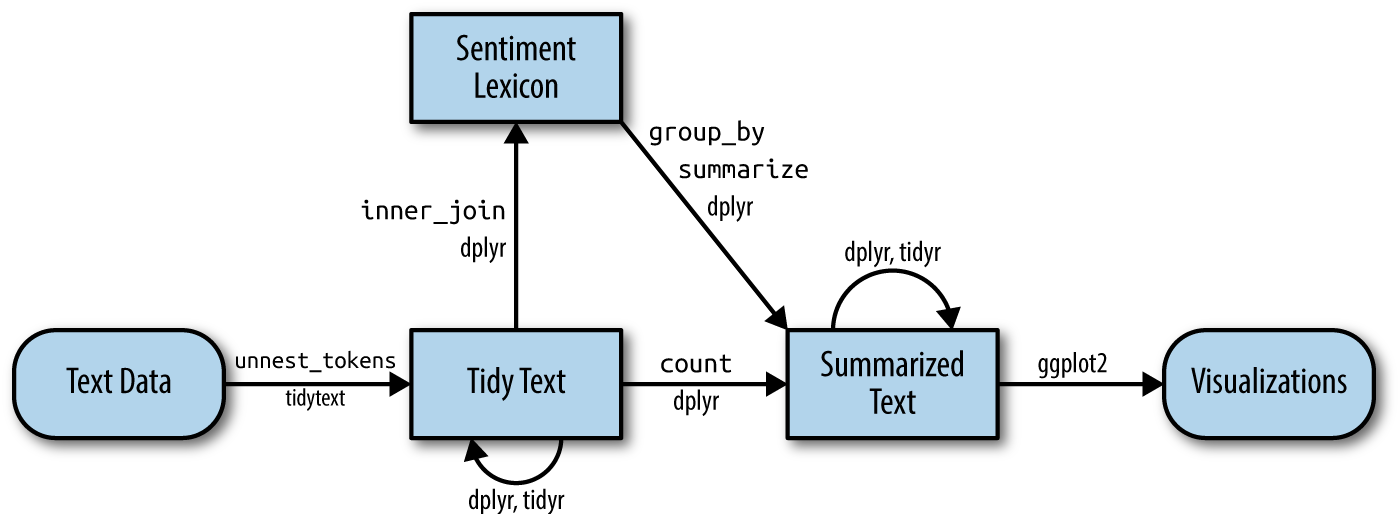
\includegraphics[width=1\linewidth]{images/tmwr_0201} 

}

\caption{A flowchart of a typical text analysis that uses tidytext for sentiment analysis. This chapter shows how to implement sentiment analysis using tidy data principles.}\label{fig:tidyflow-ch2}
\end{figure}

One way to analyze the sentiment of a text is to consider the text as a combination of its individual words and the sentiment content of the whole text as the sum of the sentiment content of the individual words. This isn't the only way to approach sentiment analysis, but it is an often-used approach, \emph{and} an approach that naturally takes advantage of the tidy tool ecosystem.

\section{\texorpdfstring{The \texttt{sentiments} datasets}{The sentiments datasets}}\label{the-sentiments-datasets}

As discussed above, there are a variety of methods and dictionaries that exist for evaluating the opinion or emotion in text. The tidytext package provides access to several sentiment lexicons. Three general-purpose lexicons are

\begin{itemize}
\tightlist
\item
  \texttt{AFINN} from \href{http://www2.imm.dtu.dk/pubdb/views/publication_details.php?id=6010}{Finn Årup Nielsen},
\item
  \texttt{bing} from \href{https://www.cs.uic.edu/~liub/FBS/sentiment-analysis.html}{Bing Liu and collaborators}, and
\item
  \texttt{nrc} from \href{http://saifmohammad.com/WebPages/NRC-Emotion-Lexicon.htm}{Saif Mohammad and Peter Turney}.
\end{itemize}

All three of these lexicons are based on unigrams, i.e., single words. These lexicons contain many English words and the words are assigned scores for positive/negative sentiment, and also possibly emotions like joy, anger, sadness, and so forth. The \texttt{nrc} lexicon categorizes words in a binary fashion (``yes''/``no'') into categories of positive, negative, anger, anticipation, disgust, fear, joy, sadness, surprise, and trust. The \texttt{bing} lexicon categorizes words in a binary fashion into positive and negative categories. The \texttt{AFINN} lexicon assigns words with a score that runs between -5 and 5, with negative scores indicating negative sentiment and positive scores indicating positive sentiment.

\begin{rmdwarning}
These lexicons are available under different licenses, so be sure that
the license for the lexicon you want to use is appropriate for your
project. You may be asked to agree to a license before downloading data.
\end{rmdwarning}

The function \texttt{get\_sentiments()} allows us to get specific sentiment lexicons with the appropriate measures for each one.

\begin{Shaded}
\begin{Highlighting}[]
\FunctionTok{library}\NormalTok{(tidytext)}

\FunctionTok{get\_sentiments}\NormalTok{(}\StringTok{"afinn"}\NormalTok{)}
\end{Highlighting}
\end{Shaded}

\begin{verbatim}
#> # A tibble: 2,477 x 2
#>    word       value
#>    <chr>      <dbl>
#>  1 abandon       -2
#>  2 abandoned     -2
#>  3 abandons      -2
#>  4 abducted      -2
#>  5 abduction     -2
#>  6 abductions    -2
#>  7 abhor         -3
#>  8 abhorred      -3
#>  9 abhorrent     -3
#> 10 abhors        -3
#> # i 2,467 more rows
\end{verbatim}

\begin{Shaded}
\begin{Highlighting}[]
\FunctionTok{get\_sentiments}\NormalTok{(}\StringTok{"bing"}\NormalTok{)}
\CommentTok{\#\textgreater{} \# A tibble: 6,786 x 2}
\CommentTok{\#\textgreater{}    word        sentiment}
\CommentTok{\#\textgreater{}    \textless{}chr\textgreater{}       \textless{}chr\textgreater{}    }
\CommentTok{\#\textgreater{}  1 2{-}faces     negative }
\CommentTok{\#\textgreater{}  2 abnormal    negative }
\CommentTok{\#\textgreater{}  3 abolish     negative }
\CommentTok{\#\textgreater{}  4 abominable  negative }
\CommentTok{\#\textgreater{}  5 abominably  negative }
\CommentTok{\#\textgreater{}  6 abominate   negative }
\CommentTok{\#\textgreater{}  7 abomination negative }
\CommentTok{\#\textgreater{}  8 abort       negative }
\CommentTok{\#\textgreater{}  9 aborted     negative }
\CommentTok{\#\textgreater{} 10 aborts      negative }
\CommentTok{\#\textgreater{} \# i 6,776 more rows}
\end{Highlighting}
\end{Shaded}

\begin{Shaded}
\begin{Highlighting}[]
\FunctionTok{get\_sentiments}\NormalTok{(}\StringTok{"nrc"}\NormalTok{)}
\end{Highlighting}
\end{Shaded}

\begin{verbatim}
#> # A tibble: 13,901 x 2
#>    word        sentiment
#>    <chr>       <chr>    
#>  1 abacus      trust    
#>  2 abandon     fear     
#>  3 abandon     negative 
#>  4 abandon     sadness  
#>  5 abandoned   anger    
#>  6 abandoned   fear     
#>  7 abandoned   negative 
#>  8 abandoned   sadness  
#>  9 abandonment anger    
#> 10 abandonment fear     
#> # i 13,891 more rows
\end{verbatim}

How were these sentiment lexicons put together and validated? They were constructed via either crowdsourcing (using, for example, Amazon Mechanical Turk) or by the labor of one of the authors, and were validated using some combination of crowdsourcing again, restaurant or movie reviews, or Twitter data. Given this information, we may hesitate to apply these sentiment lexicons to styles of text dramatically different from what they were validated on, such as narrative fiction from 200 years ago. While it is true that using these sentiment lexicons with, for example, Jane Austen's novels may give us less accurate results than with tweets sent by a contemporary writer, we still can measure the sentiment content for words that are shared across the lexicon and the text.

There are also some domain-specific sentiment lexicons available, constructed to be used with text from a specific content area. Section \ref{financial} explores an analysis using a sentiment lexicon specifically for finance.

\begin{rmdnote}
Dictionary-based methods like the ones we are discussing find the total
sentiment of a piece of text by adding up the individual sentiment
scores for each word in the text.
\end{rmdnote}

Not every English word is in the lexicons because many English words are pretty neutral. It is important to keep in mind that these methods do not take into account qualifiers before a word, such as in ``no good'' or ``not true''; a lexicon-based method like this is based on unigrams only. For many kinds of text (like the narrative examples below), there are not sustained sections of sarcasm or negated text, so this is not an important effect. Also, we can use a tidy text approach to begin to understand what kinds of negation words are important in a given text; see Chapter \ref{usenet} for an extended example of such an analysis.

One last caveat is that the size of the chunk of text that we use to add up unigram sentiment scores can have an effect on an analysis. A text the size of many paragraphs can often have positive and negative sentiment averaged out to about zero, while sentence-sized or paragraph-sized text often works better.

\section{Sentiment analysis with inner join}\label{sentiment-analysis-with-inner-join}

With data in a tidy format, sentiment analysis can be done as an inner join. This is another of the great successes of viewing text mining as a tidy data analysis task; much as removing stop words is an antijoin operation, performing sentiment analysis is an inner join operation.

Let's look at the words with a joy score from the NRC lexicon. What are the most common joy words in \emph{Emma}? First, we need to take the text of the novels and convert the text to the tidy format using \texttt{unnest\_tokens()}, just as we did in Section \ref{tidyausten}. Let's also set up some other columns to keep track of which line and chapter of the book each word comes from; we use \texttt{group\_by} and \texttt{mutate} to construct those columns.

\begin{Shaded}
\begin{Highlighting}[]
\FunctionTok{library}\NormalTok{(janeaustenr)}
\FunctionTok{library}\NormalTok{(dplyr)}
\FunctionTok{library}\NormalTok{(stringr)}

\NormalTok{tidy\_books }\OtherTok{\textless{}{-}} \FunctionTok{austen\_books}\NormalTok{() }\SpecialCharTok{\%\textgreater{}\%}
  \FunctionTok{group\_by}\NormalTok{(book) }\SpecialCharTok{\%\textgreater{}\%}
  \FunctionTok{mutate}\NormalTok{(}
    \AttributeTok{linenumber =} \FunctionTok{row\_number}\NormalTok{(),}
    \AttributeTok{chapter =} \FunctionTok{cumsum}\NormalTok{(}\FunctionTok{str\_detect}\NormalTok{(text, }
                                \FunctionTok{regex}\NormalTok{(}\StringTok{"\^{}chapter [}\SpecialCharTok{\textbackslash{}\textbackslash{}}\StringTok{divxlc]"}\NormalTok{, }
                                      \AttributeTok{ignore\_case =} \ConstantTok{TRUE}\NormalTok{)))) }\SpecialCharTok{\%\textgreater{}\%}
  \FunctionTok{ungroup}\NormalTok{() }\SpecialCharTok{\%\textgreater{}\%}
  \FunctionTok{unnest\_tokens}\NormalTok{(word, text)}
\end{Highlighting}
\end{Shaded}

Notice that we chose the name \texttt{word} for the output column from \texttt{unnest\_tokens()}. This is a convenient choice because the sentiment lexicons and stop word datasets have columns named \texttt{word}; performing inner joins and anti-joins is thus easier.

Now that the text is in a tidy format with one word per row, we are ready to do the sentiment analysis. First, let's use the NRC lexicon and \texttt{filter()} for the joy words. Next, let's \texttt{filter()} the data frame with the text from the books for the words from \emph{Emma} and then use \texttt{inner\_join()} to perform the sentiment analysis. What are the most common joy words in \emph{Emma}? Let's use \texttt{count()} from dplyr.

\begin{Shaded}
\begin{Highlighting}[]
\NormalTok{nrc\_joy }\OtherTok{\textless{}{-}} \FunctionTok{get\_sentiments}\NormalTok{(}\StringTok{"nrc"}\NormalTok{) }\SpecialCharTok{\%\textgreater{}\%} 
  \FunctionTok{filter}\NormalTok{(sentiment }\SpecialCharTok{==} \StringTok{"joy"}\NormalTok{)}

\NormalTok{tidy\_books }\SpecialCharTok{\%\textgreater{}\%}
  \FunctionTok{filter}\NormalTok{(book }\SpecialCharTok{==} \StringTok{"Emma"}\NormalTok{) }\SpecialCharTok{\%\textgreater{}\%}
  \FunctionTok{inner\_join}\NormalTok{(nrc\_joy) }\SpecialCharTok{\%\textgreater{}\%}
  \FunctionTok{count}\NormalTok{(word, }\AttributeTok{sort =} \ConstantTok{TRUE}\NormalTok{)}
\end{Highlighting}
\end{Shaded}

\begin{verbatim}
#> # A tibble: 303 x 2
#>    word        n
#>    <chr>   <int>
#>  1 good      359
#>  2 young     192
#>  3 friend    166
#>  4 hope      143
#>  5 happy     125
#>  6 love      117
#>  7 deal       92
#>  8 found      92
#>  9 present    89
#> 10 kind       82
#> # i 293 more rows
\end{verbatim}

We see mostly positive, happy words about hope, friendship, and love here. We also see some words that may not be used joyfully by Austen (``found'', ``present''); we will discuss this in more detail in Section \ref{most-positive-negative}.

We can also examine how sentiment changes throughout each novel. We can do this with just a handful of lines that are mostly dplyr functions. First, we find a sentiment score for each word using the Bing lexicon and \texttt{inner\_join()}.

Next, we count up how many positive and negative words there are in defined sections of each book. We define an \texttt{index} here to keep track of where we are in the narrative; this index (using integer division) counts up sections of 80 lines of text.

\begin{rmdtip}
The \texttt{\%/\%} operator does integer division (\texttt{x\ \%/\%\ y}
is equivalent to \texttt{floor(x/y)}) so the index keeps track of which
80-line section of text we are counting up negative and positive
sentiment in.
\end{rmdtip}

Small sections of text may not have enough words in them to get a good estimate of sentiment while really large sections can wash out narrative structure. For these books, using 80 lines works well, but this can vary depending on individual texts, how long the lines were to start with, etc. We then use \texttt{pivot\_wider()} so that we have negative and positive sentiment in separate columns, and lastly calculate a net sentiment (positive - negative).

\begin{Shaded}
\begin{Highlighting}[]
\FunctionTok{library}\NormalTok{(tidyr)}

\NormalTok{jane\_austen\_sentiment }\OtherTok{\textless{}{-}}\NormalTok{ tidy\_books }\SpecialCharTok{\%\textgreater{}\%}
  \FunctionTok{inner\_join}\NormalTok{(}\FunctionTok{get\_sentiments}\NormalTok{(}\StringTok{"bing"}\NormalTok{)) }\SpecialCharTok{\%\textgreater{}\%}
  \FunctionTok{count}\NormalTok{(book, }\AttributeTok{index =}\NormalTok{ linenumber }\SpecialCharTok{\%/\%} \DecValTok{80}\NormalTok{, sentiment) }\SpecialCharTok{\%\textgreater{}\%}
  \FunctionTok{pivot\_wider}\NormalTok{(}\AttributeTok{names\_from =}\NormalTok{ sentiment, }\AttributeTok{values\_from =}\NormalTok{ n, }\AttributeTok{values\_fill =} \DecValTok{0}\NormalTok{) }\SpecialCharTok{\%\textgreater{}\%} 
  \FunctionTok{mutate}\NormalTok{(}\AttributeTok{sentiment =}\NormalTok{ positive }\SpecialCharTok{{-}}\NormalTok{ negative)}
\end{Highlighting}
\end{Shaded}

Now we can plot these sentiment scores across the plot trajectory of each novel. Notice that we are plotting against the \texttt{index} on the x-axis that keeps track of narrative time in sections of text.

\begin{Shaded}
\begin{Highlighting}[]
\FunctionTok{library}\NormalTok{(ggplot2)}

\FunctionTok{ggplot}\NormalTok{(jane\_austen\_sentiment, }\FunctionTok{aes}\NormalTok{(index, sentiment, }\AttributeTok{fill =}\NormalTok{ book)) }\SpecialCharTok{+}
  \FunctionTok{geom\_col}\NormalTok{(}\AttributeTok{show.legend =} \ConstantTok{FALSE}\NormalTok{) }\SpecialCharTok{+}
  \FunctionTok{facet\_wrap}\NormalTok{(}\SpecialCharTok{\textasciitilde{}}\NormalTok{book, }\AttributeTok{ncol =} \DecValTok{2}\NormalTok{, }\AttributeTok{scales =} \StringTok{"free\_x"}\NormalTok{)}
\end{Highlighting}
\end{Shaded}

\begin{figure}

{\centering 
\includegraphics[width=0.9\linewidth]{02-phenotypic-data_files/figure-latex/sentimentplot-1} 

}

\caption{Sentiment through the narratives of Jane Austen's novels}\label{fig:sentimentplot}
\end{figure}

We can see in Figure \ref{fig:sentimentplot} how the plot of each novel changes toward more positive or negative sentiment over the trajectory of the story.

\section{Comparing the three sentiment dictionaries}\label{comparing-the-three-sentiment-dictionaries}

With several options for sentiment lexicons, you might want some more information on which one is appropriate for your purposes. Let's use all three sentiment lexicons and examine how the sentiment changes across the narrative arc of \emph{Pride and Prejudice}. First, let's use \texttt{filter()} to choose only the words from the one novel we are interested in.

\begin{Shaded}
\begin{Highlighting}[]
\NormalTok{pride\_prejudice }\OtherTok{\textless{}{-}}\NormalTok{ tidy\_books }\SpecialCharTok{\%\textgreater{}\%} 
  \FunctionTok{filter}\NormalTok{(book }\SpecialCharTok{==} \StringTok{"Pride \& Prejudice"}\NormalTok{)}

\NormalTok{pride\_prejudice}
\CommentTok{\#\textgreater{} \# A tibble: 122,204 x 4}
\CommentTok{\#\textgreater{}    book              linenumber chapter word     }
\CommentTok{\#\textgreater{}    \textless{}fct\textgreater{}                  \textless{}int\textgreater{}   \textless{}int\textgreater{} \textless{}chr\textgreater{}    }
\CommentTok{\#\textgreater{}  1 Pride \& Prejudice          1       0 pride    }
\CommentTok{\#\textgreater{}  2 Pride \& Prejudice          1       0 and      }
\CommentTok{\#\textgreater{}  3 Pride \& Prejudice          1       0 prejudice}
\CommentTok{\#\textgreater{}  4 Pride \& Prejudice          3       0 by       }
\CommentTok{\#\textgreater{}  5 Pride \& Prejudice          3       0 jane     }
\CommentTok{\#\textgreater{}  6 Pride \& Prejudice          3       0 austen   }
\CommentTok{\#\textgreater{}  7 Pride \& Prejudice          7       1 chapter  }
\CommentTok{\#\textgreater{}  8 Pride \& Prejudice          7       1 1        }
\CommentTok{\#\textgreater{}  9 Pride \& Prejudice         10       1 it       }
\CommentTok{\#\textgreater{} 10 Pride \& Prejudice         10       1 is       }
\CommentTok{\#\textgreater{} \# i 122,194 more rows}
\end{Highlighting}
\end{Shaded}

Now, we can use \texttt{inner\_join()} to calculate the sentiment in different ways.

\begin{rmdnote}
Remember from above that the AFINN lexicon measures sentiment with a
numeric score between -5 and 5, while the other two lexicons categorize
words in a binary fashion, either positive or negative. To find a
sentiment score in chunks of text throughout the novel, we will need to
use a different pattern for the AFINN lexicon than for the other two.
\end{rmdnote}

Let's again use integer division (\texttt{\%/\%}) to define larger sections of text that span multiple lines, and we can use the same pattern with \texttt{count()}, \texttt{pivot\_wider()}, and \texttt{mutate()} to find the net sentiment in each of these sections of text.

\begin{Shaded}
\begin{Highlighting}[]
\NormalTok{afinn }\OtherTok{\textless{}{-}}\NormalTok{ pride\_prejudice }\SpecialCharTok{\%\textgreater{}\%} 
  \FunctionTok{inner\_join}\NormalTok{(}\FunctionTok{get\_sentiments}\NormalTok{(}\StringTok{"afinn"}\NormalTok{)) }\SpecialCharTok{\%\textgreater{}\%} 
  \FunctionTok{group\_by}\NormalTok{(}\AttributeTok{index =}\NormalTok{ linenumber }\SpecialCharTok{\%/\%} \DecValTok{80}\NormalTok{) }\SpecialCharTok{\%\textgreater{}\%} 
  \FunctionTok{summarise}\NormalTok{(}\AttributeTok{sentiment =} \FunctionTok{sum}\NormalTok{(value)) }\SpecialCharTok{\%\textgreater{}\%} 
  \FunctionTok{mutate}\NormalTok{(}\AttributeTok{method =} \StringTok{"AFINN"}\NormalTok{)}

\NormalTok{bing\_and\_nrc }\OtherTok{\textless{}{-}} \FunctionTok{bind\_rows}\NormalTok{(}
\NormalTok{  pride\_prejudice }\SpecialCharTok{\%\textgreater{}\%} 
    \FunctionTok{inner\_join}\NormalTok{(}\FunctionTok{get\_sentiments}\NormalTok{(}\StringTok{"bing"}\NormalTok{)) }\SpecialCharTok{\%\textgreater{}\%}
    \FunctionTok{mutate}\NormalTok{(}\AttributeTok{method =} \StringTok{"Bing et al."}\NormalTok{),}
\NormalTok{  pride\_prejudice }\SpecialCharTok{\%\textgreater{}\%} 
    \FunctionTok{inner\_join}\NormalTok{(}\FunctionTok{get\_sentiments}\NormalTok{(}\StringTok{"nrc"}\NormalTok{) }\SpecialCharTok{\%\textgreater{}\%} 
                 \FunctionTok{filter}\NormalTok{(sentiment }\SpecialCharTok{\%in\%} \FunctionTok{c}\NormalTok{(}\StringTok{"positive"}\NormalTok{, }
                                         \StringTok{"negative"}\NormalTok{))}
\NormalTok{    ) }\SpecialCharTok{\%\textgreater{}\%}
    \FunctionTok{mutate}\NormalTok{(}\AttributeTok{method =} \StringTok{"NRC"}\NormalTok{)) }\SpecialCharTok{\%\textgreater{}\%}
  \FunctionTok{count}\NormalTok{(method, }\AttributeTok{index =}\NormalTok{ linenumber }\SpecialCharTok{\%/\%} \DecValTok{80}\NormalTok{, sentiment) }\SpecialCharTok{\%\textgreater{}\%}
  \FunctionTok{pivot\_wider}\NormalTok{(}\AttributeTok{names\_from =}\NormalTok{ sentiment,}
              \AttributeTok{values\_from =}\NormalTok{ n,}
              \AttributeTok{values\_fill =} \DecValTok{0}\NormalTok{) }\SpecialCharTok{\%\textgreater{}\%} 
  \FunctionTok{mutate}\NormalTok{(}\AttributeTok{sentiment =}\NormalTok{ positive }\SpecialCharTok{{-}}\NormalTok{ negative)}
\end{Highlighting}
\end{Shaded}

We now have an estimate of the net sentiment (positive - negative) in each chunk of the novel text for each sentiment lexicon. Let's bind them together and visualize them in Figure \ref{fig:compareplot}.



\begin{Shaded}
\begin{Highlighting}[]
\FunctionTok{bind\_rows}\NormalTok{(afinn, }
\NormalTok{          bing\_and\_nrc) }\SpecialCharTok{\%\textgreater{}\%}
  \FunctionTok{ggplot}\NormalTok{(}\FunctionTok{aes}\NormalTok{(index, sentiment, }\AttributeTok{fill =}\NormalTok{ method)) }\SpecialCharTok{+}
  \FunctionTok{geom\_col}\NormalTok{(}\AttributeTok{show.legend =} \ConstantTok{FALSE}\NormalTok{) }\SpecialCharTok{+}
  \FunctionTok{facet\_wrap}\NormalTok{(}\SpecialCharTok{\textasciitilde{}}\NormalTok{method, }\AttributeTok{ncol =} \DecValTok{1}\NormalTok{, }\AttributeTok{scales =} \StringTok{"free\_y"}\NormalTok{)}
\end{Highlighting}
\end{Shaded}

\begin{figure}

{\centering 
\includegraphics[width=0.9\linewidth]{02-phenotypic-data_files/figure-latex/compareplot-1} 

}

\caption{Comparing three sentiment lexicons using \emph{Pride and Prejudice}}\label{fig:compareplot}
\end{figure}

The three different lexicons for calculating sentiment give results that are different in an absolute sense but have similar relative trajectories through the novel. We see similar dips and peaks in sentiment at about the same places in the novel, but the absolute values are significantly different. The AFINN lexicon gives the largest absolute values, with high positive values. The lexicon from Bing et al.~has lower absolute values and seems to label larger blocks of contiguous positive or negative text. The NRC results are shifted higher relative to the other two, labeling the text more positively, but detects similar relative changes in the text. We find similar differences between the methods when looking at other novels; the NRC sentiment is high, the AFINN sentiment has more variance, the Bing et al.~sentiment appears to find longer stretches of similar text, but all three agree roughly on the overall trends in the sentiment through a narrative arc.

Why is, for example, the result for the NRC lexicon biased so high in sentiment compared to the Bing et al.~result? Let's look briefly at how many positive and negative words are in these lexicons.

\begin{Shaded}
\begin{Highlighting}[]
\FunctionTok{get\_sentiments}\NormalTok{(}\StringTok{"nrc"}\NormalTok{) }\SpecialCharTok{\%\textgreater{}\%} 
  \FunctionTok{filter}\NormalTok{(sentiment }\SpecialCharTok{\%in\%} \FunctionTok{c}\NormalTok{(}\StringTok{"positive"}\NormalTok{, }\StringTok{"negative"}\NormalTok{)) }\SpecialCharTok{\%\textgreater{}\%} 
  \FunctionTok{count}\NormalTok{(sentiment)}
\end{Highlighting}
\end{Shaded}

\begin{verbatim}
#> # A tibble: 2 x 2
#>   sentiment     n
#>   <chr>     <int>
#> 1 negative   3324
#> 2 positive   2312
\end{verbatim}

\begin{Shaded}
\begin{Highlighting}[]
\FunctionTok{get\_sentiments}\NormalTok{(}\StringTok{"bing"}\NormalTok{) }\SpecialCharTok{\%\textgreater{}\%} 
  \FunctionTok{count}\NormalTok{(sentiment)}
\CommentTok{\#\textgreater{} \# A tibble: 2 x 2}
\CommentTok{\#\textgreater{}   sentiment     n}
\CommentTok{\#\textgreater{}   \textless{}chr\textgreater{}     \textless{}int\textgreater{}}
\CommentTok{\#\textgreater{} 1 negative   4781}
\CommentTok{\#\textgreater{} 2 positive   2005}
\end{Highlighting}
\end{Shaded}

Both lexicons have more negative than positive words, but the ratio of negative to positive words is higher in the Bing lexicon than the NRC lexicon. This will contribute to the effect we see in the plot above, as will any systematic difference in word matches, e.g.~if the negative words in the NRC lexicon do not match the words that Jane Austen uses very well. Whatever the source of these differences, we see similar relative trajectories across the narrative arc, with similar changes in slope, but marked differences in absolute sentiment from lexicon to lexicon. This is all important context to keep in mind when choosing a sentiment lexicon for analysis.

\section{Most common positive and negative words}\label{most-positive-negative}

One advantage of having the data frame with both sentiment and word is that we can analyze word counts that contribute to each sentiment. By implementing \texttt{count()} here with arguments of both \texttt{word} and \texttt{sentiment}, we find out how much each word contributed to each sentiment.

\begin{Shaded}
\begin{Highlighting}[]
\NormalTok{bing\_word\_counts }\OtherTok{\textless{}{-}}\NormalTok{ tidy\_books }\SpecialCharTok{\%\textgreater{}\%}
  \FunctionTok{inner\_join}\NormalTok{(}\FunctionTok{get\_sentiments}\NormalTok{(}\StringTok{"bing"}\NormalTok{)) }\SpecialCharTok{\%\textgreater{}\%}
  \FunctionTok{count}\NormalTok{(word, sentiment, }\AttributeTok{sort =} \ConstantTok{TRUE}\NormalTok{) }\SpecialCharTok{\%\textgreater{}\%}
  \FunctionTok{ungroup}\NormalTok{()}

\NormalTok{bing\_word\_counts}
\CommentTok{\#\textgreater{} \# A tibble: 2,585 x 3}
\CommentTok{\#\textgreater{}    word     sentiment     n}
\CommentTok{\#\textgreater{}    \textless{}chr\textgreater{}    \textless{}chr\textgreater{}     \textless{}int\textgreater{}}
\CommentTok{\#\textgreater{}  1 miss     negative   1855}
\CommentTok{\#\textgreater{}  2 well     positive   1523}
\CommentTok{\#\textgreater{}  3 good     positive   1380}
\CommentTok{\#\textgreater{}  4 great    positive    981}
\CommentTok{\#\textgreater{}  5 like     positive    725}
\CommentTok{\#\textgreater{}  6 better   positive    639}
\CommentTok{\#\textgreater{}  7 enough   positive    613}
\CommentTok{\#\textgreater{}  8 happy    positive    534}
\CommentTok{\#\textgreater{}  9 love     positive    495}
\CommentTok{\#\textgreater{} 10 pleasure positive    462}
\CommentTok{\#\textgreater{} \# i 2,575 more rows}
\end{Highlighting}
\end{Shaded}

This can be shown visually, and we can pipe straight into ggplot2, if we like, because of the way we are consistently using tools built for handling tidy data frames.

\begin{Shaded}
\begin{Highlighting}[]
\NormalTok{bing\_word\_counts }\SpecialCharTok{\%\textgreater{}\%}
  \FunctionTok{group\_by}\NormalTok{(sentiment) }\SpecialCharTok{\%\textgreater{}\%}
  \FunctionTok{slice\_max}\NormalTok{(n, }\AttributeTok{n =} \DecValTok{10}\NormalTok{) }\SpecialCharTok{\%\textgreater{}\%} 
  \FunctionTok{ungroup}\NormalTok{() }\SpecialCharTok{\%\textgreater{}\%}
  \FunctionTok{mutate}\NormalTok{(}\AttributeTok{word =} \FunctionTok{reorder}\NormalTok{(word, n)) }\SpecialCharTok{\%\textgreater{}\%}
  \FunctionTok{ggplot}\NormalTok{(}\FunctionTok{aes}\NormalTok{(n, word, }\AttributeTok{fill =}\NormalTok{ sentiment)) }\SpecialCharTok{+}
  \FunctionTok{geom\_col}\NormalTok{(}\AttributeTok{show.legend =} \ConstantTok{FALSE}\NormalTok{) }\SpecialCharTok{+}
  \FunctionTok{facet\_wrap}\NormalTok{(}\SpecialCharTok{\textasciitilde{}}\NormalTok{sentiment, }\AttributeTok{scales =} \StringTok{"free\_y"}\NormalTok{) }\SpecialCharTok{+}
  \FunctionTok{labs}\NormalTok{(}\AttributeTok{x =} \StringTok{"Contribution to sentiment"}\NormalTok{,}
       \AttributeTok{y =} \ConstantTok{NULL}\NormalTok{)}
\end{Highlighting}
\end{Shaded}

\begin{figure}

{\centering 
\includegraphics[width=0.9\linewidth]{02-phenotypic-data_files/figure-latex/pipetoplot-1} 

}

\caption{Words that contribute to positive and negative sentiment in Jane Austen's novels}\label{fig:pipetoplot}
\end{figure}

Figure \ref{fig:pipetoplot} lets us spot an anomaly in the sentiment analysis; the word ``miss'' is coded as negative but it is used as a title for young, unmarried women in Jane Austen's works. If it were appropriate for our purposes, we could easily add ``miss'' to a custom stop-words list using \texttt{bind\_rows()}. We could implement that with a strategy such as this.

\begin{Shaded}
\begin{Highlighting}[]
\NormalTok{custom\_stop\_words }\OtherTok{\textless{}{-}} \FunctionTok{bind\_rows}\NormalTok{(}\FunctionTok{tibble}\NormalTok{(}\AttributeTok{word =} \FunctionTok{c}\NormalTok{(}\StringTok{"miss"}\NormalTok{),  }
                                      \AttributeTok{lexicon =} \FunctionTok{c}\NormalTok{(}\StringTok{"custom"}\NormalTok{)), }
\NormalTok{                               stop\_words)}

\NormalTok{custom\_stop\_words}
\CommentTok{\#\textgreater{} \# A tibble: 1,150 x 2}
\CommentTok{\#\textgreater{}    word        lexicon}
\CommentTok{\#\textgreater{}    \textless{}chr\textgreater{}       \textless{}chr\textgreater{}  }
\CommentTok{\#\textgreater{}  1 miss        custom }
\CommentTok{\#\textgreater{}  2 a           SMART  }
\CommentTok{\#\textgreater{}  3 a\textquotesingle{}s         SMART  }
\CommentTok{\#\textgreater{}  4 able        SMART  }
\CommentTok{\#\textgreater{}  5 about       SMART  }
\CommentTok{\#\textgreater{}  6 above       SMART  }
\CommentTok{\#\textgreater{}  7 according   SMART  }
\CommentTok{\#\textgreater{}  8 accordingly SMART  }
\CommentTok{\#\textgreater{}  9 across      SMART  }
\CommentTok{\#\textgreater{} 10 actually    SMART  }
\CommentTok{\#\textgreater{} \# i 1,140 more rows}
\end{Highlighting}
\end{Shaded}

\section{Wordclouds}\label{wordclouds}

We've seen that this tidy text mining approach works well with ggplot2, but having our data in a tidy format is useful for other plots as well.

For example, consider the wordcloud package, which uses base R graphics. Let's look at the most common words in Jane Austen's works as a whole again, but this time as a wordcloud in Figure \ref{fig:firstwordcloud}.

\begin{Shaded}
\begin{Highlighting}[]
\FunctionTok{library}\NormalTok{(wordcloud)}

\NormalTok{tidy\_books }\SpecialCharTok{\%\textgreater{}\%}
  \FunctionTok{anti\_join}\NormalTok{(stop\_words) }\SpecialCharTok{\%\textgreater{}\%}
  \FunctionTok{count}\NormalTok{(word) }\SpecialCharTok{\%\textgreater{}\%}
  \FunctionTok{with}\NormalTok{(}\FunctionTok{wordcloud}\NormalTok{(word, n, }\AttributeTok{max.words =} \DecValTok{100}\NormalTok{))}
\end{Highlighting}
\end{Shaded}

\begin{figure}

{\centering 
\includegraphics[width=0.9\linewidth]{02-phenotypic-data_files/figure-latex/firstwordcloud-1} 

}

\caption{The most common words in Jane Austen's novels}\label{fig:firstwordcloud}
\end{figure}

In other functions, such as \texttt{comparison.cloud()}, you may need to turn the data frame into a matrix with reshape2's \texttt{acast()}. Let's do the sentiment analysis to tag positive and negative words using an inner join, then find the most common positive and negative words. Until the step where we need to send the data to \texttt{comparison.cloud()}, this can all be done with joins, piping, and dplyr because our data is in tidy format.

\begin{Shaded}
\begin{Highlighting}[]
\FunctionTok{library}\NormalTok{(reshape2)}

\NormalTok{tidy\_books }\SpecialCharTok{\%\textgreater{}\%}
  \FunctionTok{inner\_join}\NormalTok{(}\FunctionTok{get\_sentiments}\NormalTok{(}\StringTok{"bing"}\NormalTok{)) }\SpecialCharTok{\%\textgreater{}\%}
  \FunctionTok{count}\NormalTok{(word, sentiment, }\AttributeTok{sort =} \ConstantTok{TRUE}\NormalTok{) }\SpecialCharTok{\%\textgreater{}\%}
  \FunctionTok{acast}\NormalTok{(word }\SpecialCharTok{\textasciitilde{}}\NormalTok{ sentiment, }\AttributeTok{value.var =} \StringTok{"n"}\NormalTok{, }\AttributeTok{fill =} \DecValTok{0}\NormalTok{) }\SpecialCharTok{\%\textgreater{}\%}
  \FunctionTok{comparison.cloud}\NormalTok{(}\AttributeTok{colors =} \FunctionTok{c}\NormalTok{(}\StringTok{"gray20"}\NormalTok{, }\StringTok{"gray80"}\NormalTok{),}
                   \AttributeTok{max.words =} \DecValTok{100}\NormalTok{)}
\end{Highlighting}
\end{Shaded}

\begin{figure}

{\centering 
\includegraphics[width=0.9\linewidth]{02-phenotypic-data_files/figure-latex/wordcloud-1} 

}

\caption{Most common positive and negative words in Jane Austen's novels}\label{fig:wordcloud}
\end{figure}

The size of a word's text in Figure \ref{fig:wordcloud} is in proportion to its frequency within its sentiment. We can use this visualization to see the most important positive and negative words, but the sizes of the words are not comparable across sentiments.

\section{Looking at units beyond just words}\label{looking-at-units-beyond-just-words}

Lots of useful work can be done by tokenizing at the word level, but sometimes it is useful or necessary to look at different units of text. For example, some sentiment analysis algorithms look beyond only unigrams (i.e.~single words) to try to understand the sentiment of a sentence as a whole. These algorithms try to understand that

\begin{quote}
I am not having a good day.
\end{quote}

is a sad sentence, not a happy one, because of negation. R packages included coreNLP \citep{R-coreNLP}, cleanNLP \citep{R-cleanNLP}, and sentimentr \citep{R-sentimentr} are examples of such sentiment analysis algorithms. For these, we may want to tokenize text into sentences, and it makes sense to use a new name for the output column in such a case.

\begin{Shaded}
\begin{Highlighting}[]
\NormalTok{p\_and\_p\_sentences }\OtherTok{\textless{}{-}} \FunctionTok{tibble}\NormalTok{(}\AttributeTok{text =}\NormalTok{ prideprejudice) }\SpecialCharTok{\%\textgreater{}\%} 
  \FunctionTok{unnest\_tokens}\NormalTok{(sentence, text, }\AttributeTok{token =} \StringTok{"sentences"}\NormalTok{)}
\end{Highlighting}
\end{Shaded}

Let's look at just one.

\begin{Shaded}
\begin{Highlighting}[]
\NormalTok{p\_and\_p\_sentences}\SpecialCharTok{$}\NormalTok{sentence[}\DecValTok{2}\NormalTok{]}
\CommentTok{\#\textgreater{} [1] "by jane austen"}
\end{Highlighting}
\end{Shaded}

The sentence tokenizing does seem to have a bit of trouble with UTF-8 encoded text, especially with sections of dialogue; it does much better with punctuation in ASCII. One possibility, if this is important, is to try using \texttt{iconv()}, with something like \texttt{iconv(text,\ to\ =\ \textquotesingle{}latin1\textquotesingle{})} in a mutate statement before unnesting.

Another option in \texttt{unnest\_tokens()} is to split into tokens using a regex pattern. We could use this, for example, to split the text of Jane Austen's novels into a data frame by chapter.

\begin{Shaded}
\begin{Highlighting}[]
\NormalTok{austen\_chapters }\OtherTok{\textless{}{-}} \FunctionTok{austen\_books}\NormalTok{() }\SpecialCharTok{\%\textgreater{}\%}
  \FunctionTok{group\_by}\NormalTok{(book) }\SpecialCharTok{\%\textgreater{}\%}
  \FunctionTok{unnest\_tokens}\NormalTok{(chapter, text, }\AttributeTok{token =} \StringTok{"regex"}\NormalTok{, }
                \AttributeTok{pattern =} \StringTok{"Chapter|CHAPTER [}\SpecialCharTok{\textbackslash{}\textbackslash{}}\StringTok{dIVXLC]"}\NormalTok{) }\SpecialCharTok{\%\textgreater{}\%}
  \FunctionTok{ungroup}\NormalTok{()}

\NormalTok{austen\_chapters }\SpecialCharTok{\%\textgreater{}\%} 
  \FunctionTok{group\_by}\NormalTok{(book) }\SpecialCharTok{\%\textgreater{}\%} 
  \FunctionTok{summarise}\NormalTok{(}\AttributeTok{chapters =} \FunctionTok{n}\NormalTok{())}
\CommentTok{\#\textgreater{} \# A tibble: 6 x 2}
\CommentTok{\#\textgreater{}   book                chapters}
\CommentTok{\#\textgreater{}   \textless{}fct\textgreater{}                  \textless{}int\textgreater{}}
\CommentTok{\#\textgreater{} 1 Sense \& Sensibility       51}
\CommentTok{\#\textgreater{} 2 Pride \& Prejudice         62}
\CommentTok{\#\textgreater{} 3 Mansfield Park            49}
\CommentTok{\#\textgreater{} 4 Emma                      56}
\CommentTok{\#\textgreater{} 5 Northanger Abbey          32}
\CommentTok{\#\textgreater{} 6 Persuasion                25}
\end{Highlighting}
\end{Shaded}

We have recovered the correct number of chapters in each novel (plus an ``extra'' row for each novel title). In the \texttt{austen\_chapters} data frame, each row corresponds to one chapter.

Near the beginning of this chapter, we used a similar regex to find where all the chapters were in Austen's novels for a tidy data frame organized by one-word-per-row. We can use tidy text analysis to ask questions such as what are the most negative chapters in each of Jane Austen's novels? First, let's get the list of negative words from the Bing lexicon. Second, let's make a data frame of how many words are in each chapter so we can normalize for the length of chapters. Then, let's find the number of negative words in each chapter and divide by the total words in each chapter. For each book, which chapter has the highest proportion of negative words?

\begin{Shaded}
\begin{Highlighting}[]
\NormalTok{bingnegative }\OtherTok{\textless{}{-}} \FunctionTok{get\_sentiments}\NormalTok{(}\StringTok{"bing"}\NormalTok{) }\SpecialCharTok{\%\textgreater{}\%} 
  \FunctionTok{filter}\NormalTok{(sentiment }\SpecialCharTok{==} \StringTok{"negative"}\NormalTok{)}

\NormalTok{wordcounts }\OtherTok{\textless{}{-}}\NormalTok{ tidy\_books }\SpecialCharTok{\%\textgreater{}\%}
  \FunctionTok{group\_by}\NormalTok{(book, chapter) }\SpecialCharTok{\%\textgreater{}\%}
  \FunctionTok{summarize}\NormalTok{(}\AttributeTok{words =} \FunctionTok{n}\NormalTok{())}

\NormalTok{tidy\_books }\SpecialCharTok{\%\textgreater{}\%}
  \FunctionTok{semi\_join}\NormalTok{(bingnegative) }\SpecialCharTok{\%\textgreater{}\%}
  \FunctionTok{group\_by}\NormalTok{(book, chapter) }\SpecialCharTok{\%\textgreater{}\%}
  \FunctionTok{summarize}\NormalTok{(}\AttributeTok{negativewords =} \FunctionTok{n}\NormalTok{()) }\SpecialCharTok{\%\textgreater{}\%}
  \FunctionTok{left\_join}\NormalTok{(wordcounts, }\AttributeTok{by =} \FunctionTok{c}\NormalTok{(}\StringTok{"book"}\NormalTok{, }\StringTok{"chapter"}\NormalTok{)) }\SpecialCharTok{\%\textgreater{}\%}
  \FunctionTok{mutate}\NormalTok{(}\AttributeTok{ratio =}\NormalTok{ negativewords}\SpecialCharTok{/}\NormalTok{words) }\SpecialCharTok{\%\textgreater{}\%}
  \FunctionTok{filter}\NormalTok{(chapter }\SpecialCharTok{!=} \DecValTok{0}\NormalTok{) }\SpecialCharTok{\%\textgreater{}\%}
  \FunctionTok{slice\_max}\NormalTok{(ratio, }\AttributeTok{n =} \DecValTok{1}\NormalTok{) }\SpecialCharTok{\%\textgreater{}\%} 
  \FunctionTok{ungroup}\NormalTok{()}
\CommentTok{\#\textgreater{} \# A tibble: 6 x 5}
\CommentTok{\#\textgreater{}   book                chapter negativewords words  ratio}
\CommentTok{\#\textgreater{}   \textless{}fct\textgreater{}                 \textless{}int\textgreater{}         \textless{}int\textgreater{} \textless{}int\textgreater{}  \textless{}dbl\textgreater{}}
\CommentTok{\#\textgreater{} 1 Sense \& Sensibility      43           161  3405 0.0473}
\CommentTok{\#\textgreater{} 2 Pride \& Prejudice        34           111  2104 0.0528}
\CommentTok{\#\textgreater{} 3 Mansfield Park           46           173  3685 0.0469}
\CommentTok{\#\textgreater{} 4 Emma                     15           151  3340 0.0452}
\CommentTok{\#\textgreater{} 5 Northanger Abbey         21           149  2982 0.0500}
\CommentTok{\#\textgreater{} 6 Persuasion                4            62  1807 0.0343}
\end{Highlighting}
\end{Shaded}

These are the chapters with the most sad words in each book, normalized for number of words in the chapter. What is happening in these chapters? In Chapter 43 of \emph{Sense and Sensibility} Marianne is seriously ill, near death, and in Chapter 34 of \emph{Pride and Prejudice} Mr.~Darcy proposes for the first time (so badly!). Chapter 46 of \emph{Mansfield Park} is almost the end, when everyone learns of Henry's scandalous adultery, Chapter 15 of \emph{Emma} is when horrifying Mr.~Elton proposes, and in Chapter 21 of \emph{Northanger Abbey} Catherine is deep in her Gothic faux fantasy of murder, etc. Chapter 4 of \emph{Persuasion} is when the reader gets the full flashback of Anne refusing Captain Wentworth and how sad she was and what a terrible mistake she realized it to be.

\section{Summary}\label{summary-1}

Sentiment analysis provides a way to understand the attitudes and opinions expressed in texts. In this chapter, we explored how to approach sentiment analysis using tidy data principles; when text data is in a tidy data structure, sentiment analysis can be implemented as an inner join. We can use sentiment analysis to understand how a narrative arc changes throughout its course or what words with emotional and opinion content are important for a particular text. We will continue to develop our toolbox for applying sentiment analysis to different kinds of text in our case studies later in this book.

  \bibliography{book.bib}

\end{document}
